\documentclass[10pt,a4paper]{report}
\usepackage[utf8]{inputenc}
\usepackage[T1]{fontenc}
\usepackage{amsmath}
\usepackage{amsfonts}
\usepackage{amssymb}
\usepackage{graphicx}
\usepackage{subfloat}
\usepackage{subfig}
\begin{document}
	\chapter{Version}
	This document is a common guide but it applies mainly to version $12$ or $v12$.
	
	\chapter{Components}
	\begin{figure}
		\subfloat[]{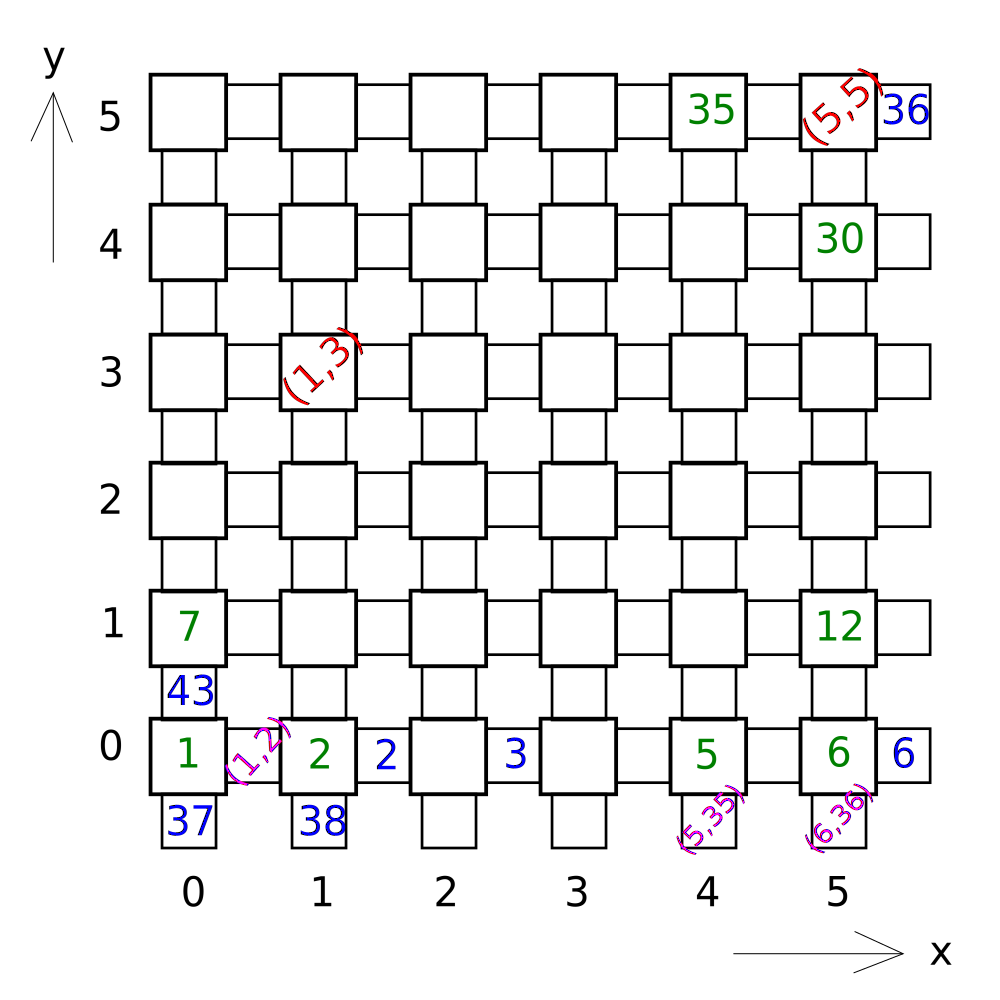
\includegraphics[width=0.8\linewidth]{fig/lattice-2.png}}
		\caption{Red color is for site index, Green color is for site id(or label), Magenta color is for bond index, Blue color is for bond id (or label).}
	\end{figure}
	\section{Site}
	\begin{enumerate}
		\item $id$ or $label$
		\item $group\_id$
		\item Index
		\item Relative Index with respect to 
	\end{enumerate}
	\section{Bond}
\begin{enumerate}
	\item $id$ or $label$
	\item $group\_id$ which can coincide with site group id
	
	\item Index. $(a,b)$ where $a$ is the $id$ of one site and $b$ is the id of another site.
\end{enumerate}
	\section{Lattice}
	\section{Cluster}
\end{document}